\documentclass[10pt,oneside,a4paper]{article}
\usepackage[left=2cm,right=2cm,top=2cm,bottom=1cm,includeheadfoot]{geometry}
\usepackage{ngerman}
\usepackage[utf8]{inputenc}
% \usepackage{amsfonts,amssymb,amsmath,cancel,graphicx,textcomp}
\usepackage{amsfonts,amssymb,amsmath,graphicx,textcomp}
\usepackage{float}
\usepackage{color,xcolor}
\usepackage{url}
\usepackage{hyperref}
\usepackage{listings}
\usepackage{tikz}
\usepackage{fancyhdr}
\usepackage{gensymb}
\usepackage[section]{placeins}
\usetikzlibrary{arrows,shapes,snakes,automata,backgrounds,petri,positioning}

\hypersetup{
    colorlinks,
    citecolor=black,
    filecolor=black,
    linkcolor=black,
    urlcolor=black
}

\pagestyle{fancy}
\fancyhf{}
\fancyhead[L]{crash override : \\Steve Dierker, Semjon Kerner, Artur Jeske}
\fancyhead[C]{"Ubungsblatt 10}
\fancyhead[R]{Seite \thepage}
\renewcommand{\headrulewidth}{0.5pt}

% lstlisting mit Zeilennummerierung und grauen Kommentaren, Zeilenumbruch, etc. pp.
\lstset{
  numbers=left, numberstyle=\tiny, numbersep=5pt,
  tabsize=2,
  breaklines=true, breakindent=0pt, postbreak=\mbox{$\rightarrow\ \ $},
  showstringspaces=false,
  extendedchars=false,
  basicstyle=\small\ttfamily,
  commentstyle=\color{black!40},
  stringstyle=\color{black!40!blue},
  keywordstyle=\color{black!40!green}
}

% Komma Abstände bei Tausendern/Dezimalzahlen ans dt. anpassen
\mathcode`,="013B
\setlength{\parindent}{0em}
\setlength{\parskip}{0.5em}

\begin{document}
  \section{Closest Point with Prediction (4 Points)}
    \begin{figure}[h]
      \centering
      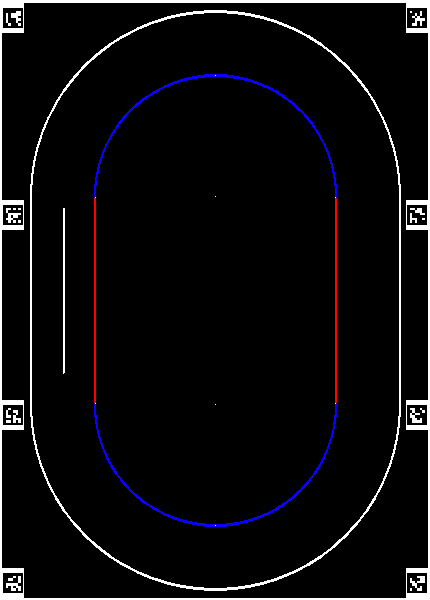
\includegraphics[scale=0.5]{pictures/map.png}
      \caption{Karte mit eingezeichneten Abschnitten.}
    \end{figure}
    \begin{itemize}
      \item{Aufgabe:} Die Aufgabenstellung war ausgehend vom closest point zwischen Linie 1 und 2 den Punkt in der Distanz voraus zu berechnen, der entsprechend entlang Wegstrecke vom Auto liegt, im besten Fall w"urde das Auto in der Mitte der beiden Linien fahren. (Auto ist zum Verst"andnis hier der Ausgangspunkt)
    \end{itemize}
    \begin{itemize}
      \item Wir bestimmen zun"achst auf welchem Abschnitt das Auto sich befindet, befinden wir uns im roten Abschnitt auf der rechten Seite (siehe Abbildung 1) , so ist das der einfachste Fall. 
      Entsprechend ob wir als Parameter Linie 1 oder 2 bekommen, addieren wir zur x Koordinate von der inneren Linie die entsprechende Liniendicke. Und von y Koordinate des Autos ziehen wir die gew"unschte Distanz ab. So erhalten wir einen Punkt, der entlang der Wegstrecke in der Distanz liegt. 
    \end{itemize}
    \begin{itemize}
      \item Befinden wir uns im roten Abschnitt auf der linken Seite, so ist die Berechnung analog zu oben.
    \end{itemize}
        \begin{itemize}
      \item Erkl"arungen zu den Kreisen folgen.
    \end{itemize}
    
    \begin{figure}[h]
      \centering
      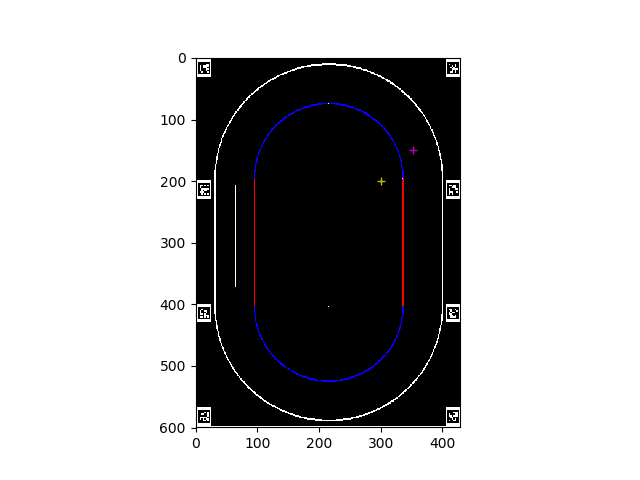
\includegraphics[scale=1.0]{pictures/u10_Figure_1.png}
      \caption{Auto in gelb, Punkt in der Distanz in Pink}
    \end{figure}
    \begin{itemize}
      \item Point(3,1) on lane 1 and distance 0.5m:
      \item ('Car point:', array([300, 200]))
      \item ('Prediction:', array([352, 150]))

    \end{itemize}
    
    Quellcode:
    \url{https://github.com/bigzed/model_car/blob/version-4.0/texinput/src/closestpointwithprediction.py}

    
  \section{Follow lane with ceiling camera GPS (6 Points)}
    Als erstes haben wir die gegebenen Koordinaten von Metern in Pixel umgerechnet, wobei \( 1m
    \equiv 100px \equiv 100cm \).

\end{document}
